\section{Implementierung der Delivery Queue} \label{dlq}

Die \textit{Delivery Queue} enthält alle Nachrichten, die an den Leser ausgeliefert werden dürfen. Sie hat einen begrenzten Speicher zur Verfügung, welcher nicht überschritten werden darf. Dieser wird bei Initialisierung der Queue übergeben und innerhalb der Queue gespeichert. Die Nachrichten werden in der \textit{Delivery Queue} in einem \textit{First-In First-Out} Speicher abgelegt. Die Nachricht die als erstes eingefügt wird, verlässt dementsprechend als erstes wieder die Liste (siehe Abbildung \ref{fig:fifo}).

\begin{figure}[htbp]
\begin{center}
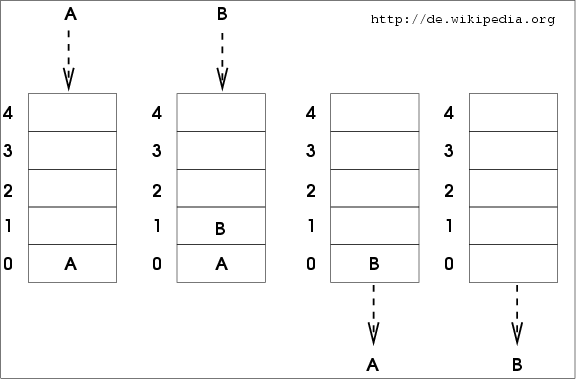
\includegraphics[scale=0.4]{Latex/Bilder/FIFO_PEPS.png}
\caption[First In First Out]{FIFO\footnotemark}\label{fig:fifo}
\end{center}
\end{figure}
\footnotetext{\url{https://de.wikipedia.org/wiki/First_In_–_First_Out}}

Dafür werden die neuen Elemente immer an die Liste angehängt, so dass die Nachricht mit der kleinsten Nummer immer an letzter Stelle eingefügt wird. Hierfür bietet sich in Erlang das Anfügen an. 

\begin{lstlisting}
NewDLQ = OldDLQ ++ [NewMessage]
\end{lstlisting}

In dieser Funktion werden zwei Listen zu einer kombiniert. Das zweite Element muss als Liste übergeben werden. Es ist mit der Struktur \textit{NewMessage = [NNr, Msg, TSclientout, TShbqin, TSdlqin]} zwar schon eine Liste, aber weil die Nachricht als ein Element eingefügt werden soll, muss es als Liste mit nur einem Element angefügt werden werden. 
Die Liste wird aufsteigend sortiert, da theoretisch genauso viele Elemente in die Liste eingefügt, wie auch wieder aus der Queue gelöscht werden. 

Ein Problem bei der \textit{Delivery Queue} stellt die vorgegebene maximale Größe dar. Diese kann nicht im Speicherplatz reserviert werden (keine In-Place Lösungen in Erlang), wie zum Beispiel über ein malloc in C oder über ein Attribut wie in Java. Die Größe muss im Prozess der Queue oder direkt in der Queue gespeichert werden.
Die erste Möglichkeit zur Speicherung der Größe bietet aber viele Fehlerquellen. Die Implementierung würde in Teilen wie folgt aussehen:
\begin{lstlisting}
spawn(fun() -> loop(Size, Datei, 0) end).

loop(MaxSize, Datei, ActSize) -> 
    receive 
        {From, getVariables} -> 
            From ! {reply, {MaxSize, Datei, ActSize}}
            loop(MaxSize, Datei, ActSize);
        {From, setVariables, {NewMaxSize, NewDatei, NewActSize}}
            From ! {reply, variablesSet}
            loop(NewMaxSize, NewDatei, NewActSize)
    end.
\end{lstlisting}

Über die Schnittstelle \textit{\{self(), getVariables\}} und \textit{\{self(), setVariables, \{NewMaxSize, NewDatei, NewActSize\}\}} können nun sowohl von der \textit{Holdback Queue} als auch von der \textit{Delivery Queue} aus das Limit der \textit{Delivery Queue}, die aktuelle Größe und die Logging Datei gelesen und geschrieben werden. Die \textit{Delivery Queue} wäre somit eine zum Teil entfernte abstrakte Datenstruktur. 
Ein Problem, welches nach der Implementierung entstanden ist, war das sehr aufwändige Debuggen von Fehlern oder Aufrufen innerhalb der Delivery Queue. 

Eine einfachere Lösung wäre das Speichern der Variablen innerhalb der Queue. 
Diese neue Queue hat die Struktur eines Tupels mit drei Elementen. Zum einen die maximale und die aktuelle Größe und zum anderen die eigentliche Queue in Form einer Liste - also \textit{DLQ = \{MaxSize, ActSize, [Msg1, Msg2, ...]\}}. So werden mögliche Fehler, welche durch Nebenläufigkeiten entstehen können, eliminiert. \\
Im Folgenden wird mit der zweiten Lösung, also der Speicherung der Elemente innerhalb der Delivery Queue als Tupel, gearbeitet.

\subsection{initDLQ}

In der Initalisierungfunktion der Delivery Queue wird die Queue erzeugt. Die Funktion hat den Aufruf \textit{initHBQ} und bekommt die maximale Größe und die Logging Datei mit übergeben. 
Nach erfolgreicher Initialisierung wird die Initialisierungsgröße der Delivery Queue geloggt und ein Tupel mit den Elementen \textit{MaxSize}, \textit{ActSize} und der eigentlichen Queue zurückgegeben.

\subsection{delDLQ}

Die \textit{Delivery Queue} wird in dieser Implementierung nicht als entfernte abstrakte Datenstruktur umgesetzt. Es muss dementsprechend kein Prozess beendet werden. Die Funktion gibt beim Aufruf \textit{ok} zurück.

\subsection{expectedNr}

Diese Funktion liefert die Nachrichtennummer die als nächstes in der \textit{Delivery Queue} gespeichert werden kann. Diese ist die größte enthaltene Nummer um eins erhöht. Die größte Nummer ist stets das letzte Element der Delivery Queue. Es wird rekursiv eine Teilliste der Queue aufgerufen und das erste Element dieser gespeichert, bis die Teilliste leer ist (siehe getLastElem/1). 
\begin{lstlisting} 
getLastElem([[NNr, _Msg, _TSclientout, _TShbqin, _TSdlqin]|[]]) -> NNr;
getLastElem([_Head|Tail]) -> getLastElem(Tail).
\end{lstlisting}

\subsection{push2DLQ}

Diese Funktion wird von der \textit{Holdback Queue} über die zugehörige Schnittstelle \textit{\{self(), \{request, pushHBQ, Msg\}\}} aufgerufen.

Die Funktion \textit{push2DLQ} speichert die übergebene Nachricht in der \textit{Delivery Queue}. Da die Queue bereits sortiert ist und das letzte Element in der Queue das Größte ist, wird das neue Element mit Zeitstempel an die Liste angefügt. 
Bei jedem Funktionsaufruf wird die maximale Größe mit der aktuellen Größe verglichen. Wenn die Delivery Queue die maximale Größe erreicht hat, dann wird beim Einfügen eines neuen Elements das Älteste gelöscht. Dies kann in Erlang sehr effizient umgesetzt werden. Durch die Aufteilung der Liste in Startelement und Restliste kann zum Löschen des ersten Elements einfach mit der Restliste weitergearbeitet werden. 

\begin{figure}[htbp]
\begin{center}
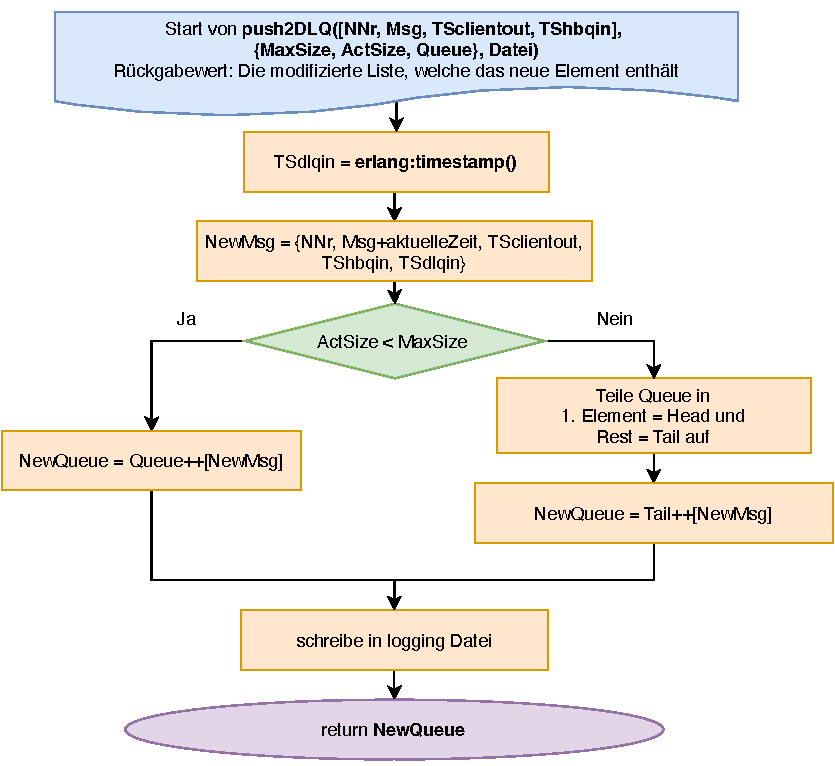
\includegraphics[scale=0.65]{Latex/Bilder/push2DLQ.pdf}
\caption{pushDLQ}\label{fig:pushDLQ}
\end{center}
\end{figure}

\subsection{deliverMSG}

Diese Funktion sendet die im Parameter übergebene Nachrichtennummer an die übergebene Prozess ID des Clients. Dafür wird durch die Elemente der Delivery Queue gelaufen, bis das Element entweder gefunden wurde oder das übergebene Element größer ist. 

\begin{lstlisting}
getMSGAtMSGNr(_MSGNr, []) -> [-1,nokb,0,0,0];
getMSGAtMSGNr(MSGNr, [[NNr, Msg, TSclientout, TShbqin, TSdlqin]|_Tail]) when MSGNr =< NNr-> 
    [NNr, Msg, TSclientout, TShbqin, TSdlqin];
getMSGAtMSGNr(MSGNr, [_Head|Tail]) -> getMSGAtMSGNr(MSGNr, Tail).
\end{lstlisting}

In obiger Funktion ist das rekursive Durchlaufen der Liste gezeigt. Der Funktion wird eine Liste übergeben, in diesem Falle die \textit{Delivery Queue}. Daraufhin wird von dieser Liste so oft das erste Element abgeschnitten, bis eine der beiden Abbruchbedingungen eintreffen. Anhand von \textit{Pattern Matching} kann verglichen werden, ob die Liste leer ist oder ob die erste Nachricht der übergebenen Liste größer gleich der gesuchten Nachrichtennummer ist.
Gelöscht werden die Elemente aus der Delivery Queue allerdings erst, sobald diese ihre maximale Größe erreicht hat.
Das eigentliche Senden der Nachricht an den Clienten findet innerhalb der Delivery Queue statt. \\Der Aufruf hat den Aufbau:
\textit{ClientPID ! \{reply,SendMessage,Terminated\}}

Um den gesamten Prozess terminieren zu können, wird der Delivery Queue von der Holdback Queue mitgeteilt ob diese noch Elemente enthält. Wenn das nicht mehr der Fall ist wird die Nachricht \textit{[-1,nkob,0,0,0]} mit einem weiteren Parameter \textit{true} übergeben.

\subsection{listDLQ}

Die Funktion gibt eine Liste mit den Nummern der in der \textit{Delivery Queue} enthaltenden Nachrichten zurück. Diese Nummern sind nach aufsteigender Größe sortiert, da am Kopf der Queue angefangen wird. Die Reihenfolge der Liste ist eingehalten. 

\subsection{lengthDLQ}

Diese Funktion gibt die Anzahl der in der \textit{Delivery Queue} enthaltenden Nachrichten zurück. Dafür wird die im Tupel der \textit{Delivery Queue} enthaltende Variable \textit{ActSize} zurückgegeben. 